\documentclass[a4paper,12pt]{article}
\usepackage[T1]{fontenc}
\usepackage[utf8]{inputenc}
% Pas de \usepackage[french]{babel} : il faut texlive-lang-french (french.ldf).
% T1 + utf8 suffisent pour é, è, à, ô, etc.
\usepackage{graphicx}
\graphicspath{ {./imgs/} }
\usepackage{fancyhdr} % For headers and footers
\usepackage{geometry}
\usepackage{longtable} % For long tables that can span multiple pages
\usepackage{array}     % For better column formatting
\usepackage{hyperref} % en dernier (liens cliquables)

% Adjust margins
\geometry{
    top=4cm, 
    bottom=2.5cm, 
    left=2.5cm, 
    right=2.5cm,
    headheight=3cm, % Ensures sufficient space for header content
    headsep=0.5cm,
    }

% Define the custom headers
\fancypagestyle{firstpage}{% First page header style
    \fancyhf{} % Clear all header/footer fields
    \fancyhead[L]{%
        
\includegraphics[height=1.5cm]{heig_logo.png} \\
    }
    \fancyhead[R]{%
        
\includegraphics[height=1.5cm]{reds_logo.png} \\
    }
    \fancyfoot{} % No footer on the first page
}

% Define other pages style
\fancypagestyle{otherpages}{%
    \fancyhf{}
    \fancyhead[L]{%
        
\includegraphics[height=1.5cm]{heig_logo.png} \\
    }
    \fancyhead[R]{%
        \small Laboratoire 5 : IP AXI4-Lite avec FPGA I/O \\
        Urs Behrmann \\
    }
    \fancyfoot[C]{\small page \thepage}
}

\author{Urs Behrmann}

\setlength{\parskip}{1em} % Définit un espace entre chaque paragraphe
\setlength{\parindent}{0pt} % Optionnel : enlève l'indentation des paragraphes

\begin{document}

\emergencystretch=1em % Ajoute une flexibilité d'espacement

% First page content
\thispagestyle{firstpage}


\vspace*{2cm}
\begin{center}
    \Huge Laboratoire 5 \\
    \vspace{0.2cm}
    \Large IP AXI4-Lite avec FPGA I/O\\
    \vspace{1cm}
    \small Départements : TIC\\
    Unité d'enseignement SCF\\
\end{center}

\vspace{9cm}

\renewcommand{\arraystretch}{1.5} % Adjust row height

\begin{flushleft} % Left-align the table
    \begin{tabular}{@{}l l@{}}
        \textbf{Auteur :}        & \textbf{Urs Behrmann} \\
        \textbf{Professeurs :}   & \textbf{Alberto Dassatti} \\
                                 & \textbf{Yann Thomas} \\
        \textbf{Assistant :}     & \textbf{Clément Dieperink} \\
        \textbf{Classe :}        & \textbf{SCF} \\
        \textbf{Salle de labo :} & \textbf{A07} \\
        \textbf{Date :}          & \textbf{01.04.2026} \\
    \end{tabular}
\end{flushleft}

\newpage

% Apply the other pages style
\pagestyle{otherpages}

\renewcommand{\contentsname}{Table des matières}
\tableofcontents

\newpage

\section{Introduction}

Ce rapport décrit le laboratoire 5 : une IP avec interface AXI4-Lite sur le bus léger HPS--FPGA, reliée aux entrées/sorties de la carte DE1-SoC (boutons, switchs, LEDs, afficheurs 7 segments).

\section{Ajout de l'IP AXI4-Lite dans Platform Designer}

J'ai créé un nouveau composant dans le Component Editor à partir du fichier \texttt{axi4lite\_slave.vhd}. Il faut lier les signaux du fichier VHDL aux interfaces attendues par Qsys : AXI4-Lite esclave, horloge, reset, et conduit pour les entrées/sorties vers le FPGA.

La figure~\ref{fig:block} montre le symbole du bloc de l'IP. Les figures~\ref{fig:param} et~\ref{fig:sig} montrent les paramètres (largeur des bus) et le placement des signaux dans les interfaces. La figure~\ref{fig:sys} montre le système \texttt{qsys\_system} avec le HPS, l'horloge, et l'instance \texttt{AXI4Lite\_0} connectée au maître léger AXI.

\begin{figure}[htbp]
    \centering
    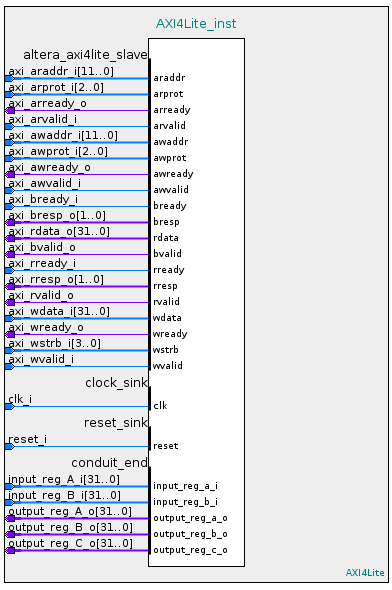
\includegraphics[width=0.45\textwidth]{axi4Lite_hw_block_symbol.png}
    \caption{Symbole du composant AXI4-Lite.}
    \label{fig:block}
\end{figure}

\begin{figure}[htbp]
    \centering
    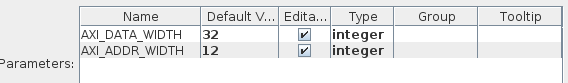
\includegraphics[width=0.55\textwidth]{axi4Lite_hw_parameters.png}
    \caption{Paramètres de l'IP (largeur d'adresse et de données).}
    \label{fig:param}
\end{figure}

\begin{figure}[htbp]
    \centering
    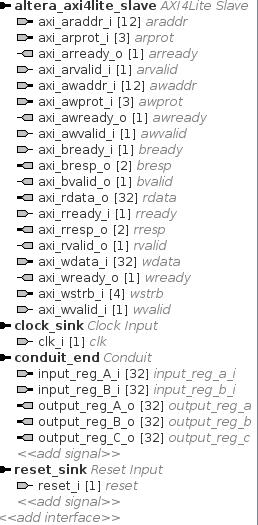
\includegraphics[width=0.30\textwidth]{axi4Lite_hw_signals_interfaces.png}
    \caption{Signaux et interfaces (AXI4-Lite, horloge, reset, conduit).}
    \label{fig:sig}
\end{figure}

\begin{figure}[htbp]
    \centering
    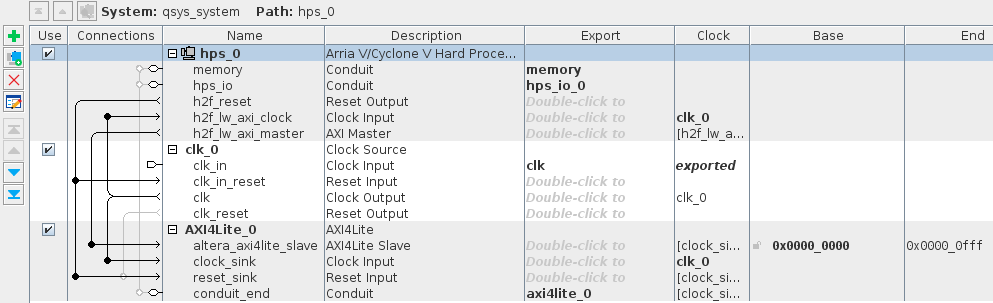
\includegraphics[width=0.95\textwidth]{axi4Lite_hw_system_contents.png}
    \caption{Contenu du système Qsys : connexions et adressage.}
    \label{fig:sys}
\end{figure}

\newpage

Après chaque modification du VHDL ou du composant, j'ai régénéré les fichiers HDL du système, puis recompilé le projet Quartus. Le fichier \texttt{DE1\_SoC.qsf} inclut le \texttt{.qip} généré et le fichier \texttt{DE1\_SoC\_top.vhd} relie les signaux du conduit aux broches de la carte (keys, SW, LEDR, HEX).

\section{Plan d'adresse de l'IP}

Les registres sont alignés sur 32 bits. Les adresses sont des \emph{décalages} par rapport à la base du périphérique sur le bus (souvent \texttt{0xFF200000} pour le pont léger).

\begin{center}
\begin{tabular}{|l|l|l|}
\hline
\textbf{Décalage} & \textbf{Rôle} & \textbf{Lecture / écriture} \\
\hline
\texttt{0x00} & Constante \texttt{0xBADB100D} (identification) & R \\
\texttt{0x04} & Registre de test & RW \\
\texttt{0x08} & État des boutons (keys) & R \\
\texttt{0x0C} & Capture de fronts sur les boutons & RW \\
\texttt{0x10} & État des switchs & R \\
\texttt{0x14} & LEDs (sortie) & RW \\
\texttt{0x18} & Set LEDs (écrire 1 met le bit à 1) & W \\
\texttt{0x1C} & Clear LEDs (écrire 1 met le bit à 0) & W \\
\texttt{0x20} & Afficheurs HEX3 à HEX0 & RW \\
\texttt{0x24} & Afficheurs HEX5 et HEX4 & RW \\
\hline
\end{tabular}
\end{center}

\section{Programme C}

Le programme lit d'abord la constante et compare avec la valeur attendue. Il écrit une valeur dans le registre de test et la relit pour vérifier que les accès mémoire fonctionnent.

Ensuite, dans une boucle infinie, il utilise le registre de capture de fronts sur les boutons : chaque action sur une touche déclenche une petite logique (valeur interne liée aux switchs, incrément, décrément, remise à zéro). Selon si l'opération est ``légale'' ou non, il allume ou éteint les LEDs avec les registres set/clear. Il affiche la valeur sur les afficheurs 7 segments.

\section{Difficultés rencontrées}

J'ai eu beaucoup de difficultés avec l'IP au début. Dans le fichier TCL du Component Editor, les noms des ports pour l'interface AXI4-Lite ne correspondaient pas exactement aux noms dans mon entity VHDL (\texttt{clk\_i}, \texttt{axi\_awaddr\_i}, etc.). Du coup, la synthèse et l'analyse Quartus échouaient avec des erreurs du type ``port inexistant''.

J'ai dû aligner les noms dans le TCL sur le VHDL, puis régénérer plusieurs fois les fichiers Qsys et refaire la compilation jusqu'à ce que tout soit cohérent. C'était long mais ça m'a appris à bien vérifier la correspondance entre Platform Designer et le code RTL.

\section{Tests sur la carte}

J'ai programmé le FPGA avec le fichier \texttt{.sof}, chargé le preloader pour le HPS, puis lancé le programme depuis Arm Development Studio. J'ai vérifié sur la carte Cyclone V (DE1-SoC) que les affichages \texttt{printf} apparaissaient, que les LEDs et les HEX réagissaient aux boutons et aux switchs, et que le comportement correspondait au cahier des charges du laboratoire.

\section{Utilisation d'outil IA}

Pour ce rapport, j'ai utilisé l'assistant \emph{Claude Sonnet} pour corriger la grammaire et l'orthographe du rapport. Le fond technique reste le mien ; seule la forme du français a été améliorée.

\end{document}